\section{CONDICION III} 

\vspace{16mm} %5mm vertical space
\begin{center}
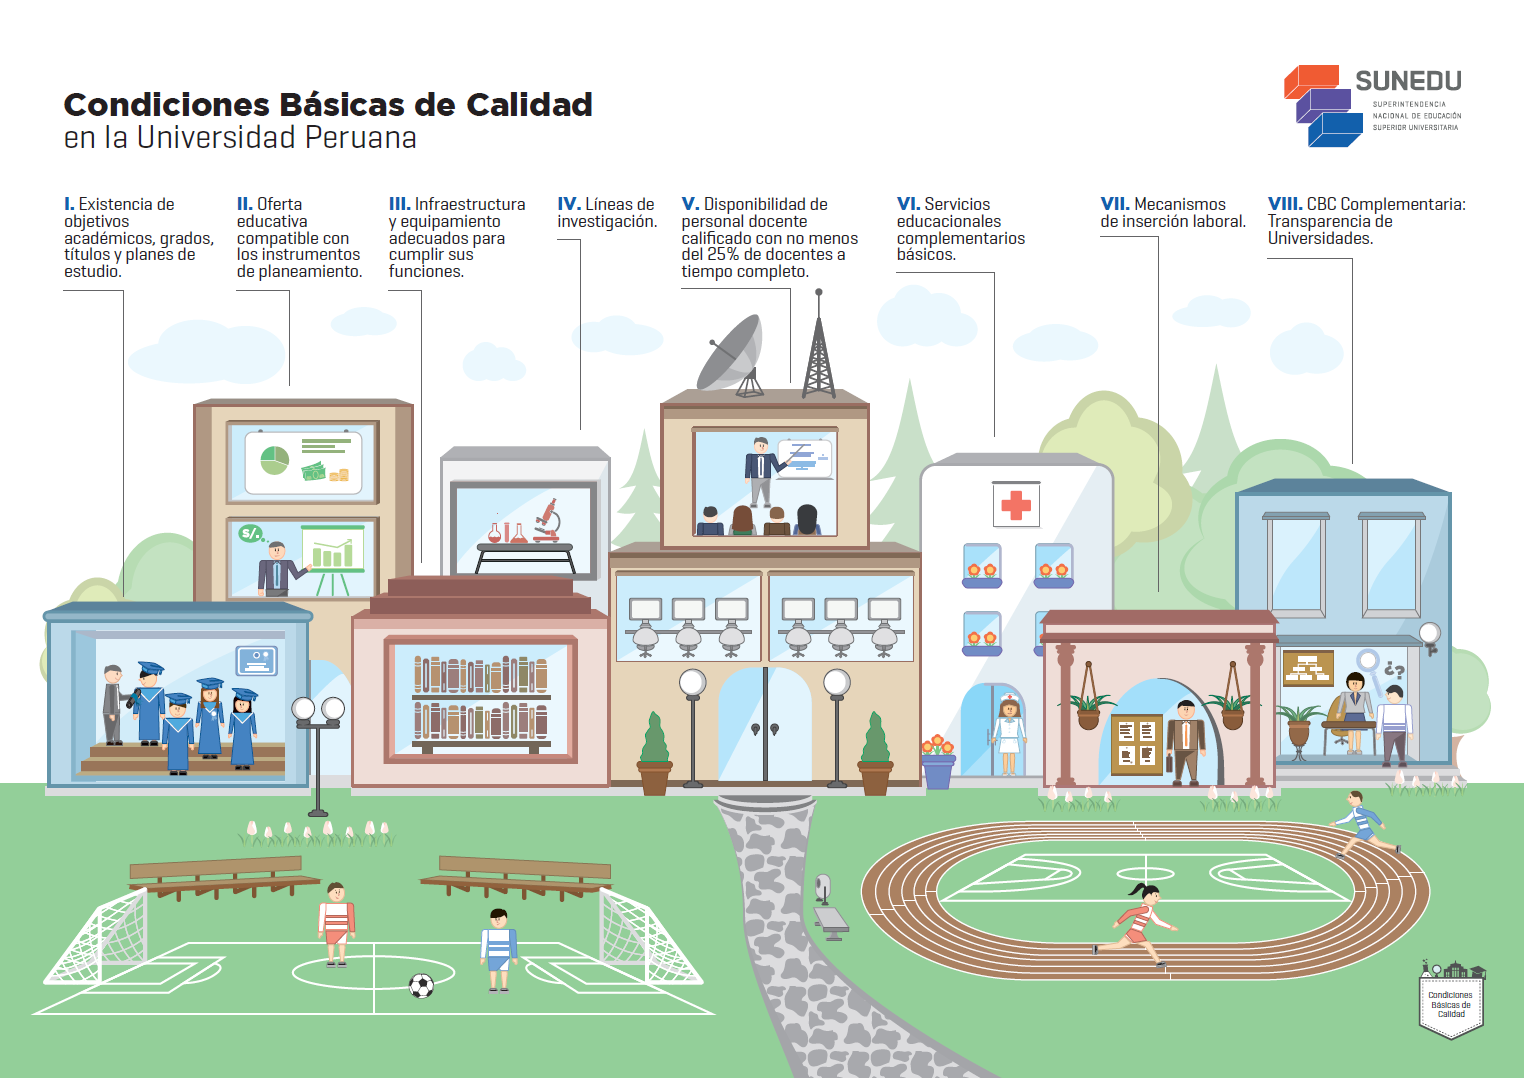
\includegraphics[width=17cm]{./Imagenes/002}
\end{center}	
\vspace{7mm} %3mm vertical space

\textbf{CONDICION III: Infraestructura y equipamiento adecuado al cumplimiento de sus funciones (aulas, bibliotecas, laboratorios, entre otros)}\\
-	ubicación de la FCAC. de acuerdo al certificad o Registral Inmobiliario, y el certificado de numeración de Finca, se encuentra ubicado en: \\
-	Universidad Privada de Tacna con que documentos como medio de verificación acredita la posesión de su local \\
-	El Reglamento interno de seguridad y salud en el trabajo y protocolos de seguridad, que tiene la Universidad Peruana los Andes, mediante qué documento 		ha sido aprobado 17. El Organigrama del comité de Seguridad y Salud en el trabajo que adopto la UPLA. está conformado por\\ 
-	Para el componente III.5 DISPONIBILIDAD DE SERVICIOS PUBLICOS, INDICADOR 21: DISPONIBILIDAD DE AGUA POTABLE Y DESAGÜE, el medio de 			verificación que se acogió la Universidad \\
-	Los ambientes para docentes de acuerdo al medio de verificación MV1: formato de licenciamiento C8, donde se registra información de la ubicación de los 			ambientes para docentes en el local de la universidad.\\

